% !TeX root = ../main.tex
% Add the above to each chapter to make compiling the PDF easier in some editors.
\graphicspath{{./figures/ch3/}}

\chapter{Experimental Design}\label{chapter:experiment}
In this chapter I first describe the data of the German spectrum auction from 2015. Afterwards, a value model is introduced that was built from the insights of the data analysis and external resources to describe the valuation of each bidder in the auction. The value model serves as a cornerstone of the simulation in \autoref{chapter:simulation}. In the last section I describe on which basis the performance of different auction formats can be compared.

\section{Data from the German Spectrum Auction 2015}
To simulate the German spectrum auction "Mobiles Breitband - Projekt 2016" (MBP16, see \autoref{sec:MBP16}) a value model needs to be derived for each bidder in the auction. To achieve that, the respective data was analysed to give insights into bidding behaviour and valuation.

\subsection{Data Aquisition}
The German Federal Network Agency (BNetzA) made the MBP16 data available to the public via their website\footnote{\url{http://www.bundesnetzagentur.de/DE/Sachgebiete/Telekommunikation/Unternehmen_Institutionen/Frequenzen/OeffentlicheNetze/Mobilfunknetze/Projekt2016/projekt2016-node.html} (accessed on 11/07/2016)}.
The data contains the highest bidder and the winning bid for each block in each round, as well as the the summed value of all retracted bids (see an example in \autoref{fig:r181data}). During the auction every bidder could see the bids placed by their competitors after each round ended \cite{Bundesnetzagentur2015}. This data is not contained in the public data set.

\begin{figure}[h]
\centering
\includegraphics[scale=0.45]{Runde181.png}
\caption{Example of the available bidding data} \label{fig:r181data}
\end{figure}

As the round data was published as image files, there was a need to systematically extract the information from the images and save it to a suitable data format. To achieve this, a Python script loaded all the images and used Optical Character Recognition (OCR), a computer vision algorithm for pattern recognition, to scan them. Afterwards, all the data was written into a CSV file.

%TODO figure necessary?
\begin{figure}[]
\centering
\includegraphics[scale=0.4]{ocr_process.png} %TODO take svg file instead
\caption{The OCR process} \label{fig:ocr_process}
\end{figure}

\subsection{Data Analysis}
Now, using the processed data I could have a look the bidding behaviour and derive insights for the value model. The paper of \citeauthor{Bichler2016} states that three different bidding phases can be found during the German Auction: the coordination phase, the competition phase and the end phase. Analysing the bids submitted during the auction, these phases could be shown using the data.  

Supporting in the process will be \autoref{fig:whowinswhat}, which visualises the different phases by showing which bidder placed the highest bids in each round, thus temporarily winning the corresponding frequency block. Additionally, \autoref{fig:meanBidsOverTime} shows the development of the mean bids by spectrum submitted by each bidder over the course of the auction to give an overview of the price progression.

\begin{figure}[h]
	\centering
	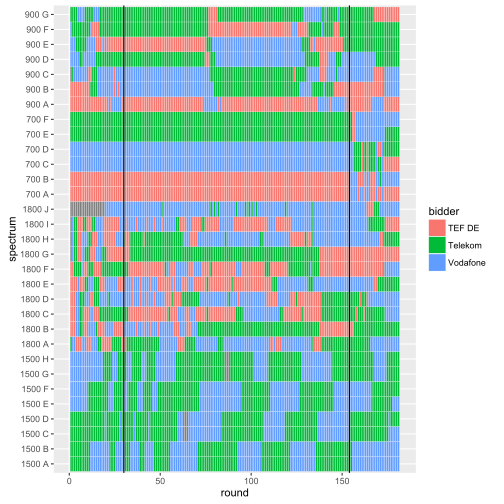
\includegraphics[scale=0.6]{bidders_who_wins_what.pdf}
	\caption{Block winner per round} \label{fig:whowinswhat}
\end{figure}


\begin{figure}[h]
	\centering
	\includegraphics[scale=0.6]{mean_bids_all_bidders.pdf}
	\caption{Development of mean bids per spectrum over time, bids in thousand EUR} \label{fig:meanBidsOverTime}
\end{figure}

In this following segment I will give a quick overview of the course of the bidding behaviour according to \citeauthor{Bichler2016}. The \textbf{coordination phase} reached from the beginning of the auction until round 30. It was marked by a careful search for possible allocations that would satisfy all the bidders which resulted in cooperative bidding behaviour, hence the naming. A distinctive feature of this phase was that prices only rose slowly, trying to signal possible mutually compatible allocations between the bidders. An interesting behaviour can be seen in the 700 MHz band. All three bidders placed bids on two blocks in the segment. As can be seen in \autoref{fig:whowinswhat}, over the course of this phase (and as we will see later, much longer than that) no new bids were placed after the initial bids in the first round, which resulted in stable prices and indicating a lack of excess demand and a demand equilibrium. In the other bands, the bidders tried to communicate their demand and signal a potential overall allocation. At the end of this phase, the total revenue over all items was at EUR 2 billion.

The \textbf{competition phase}, reaching from round 31 to 154, started with an excess demand of 2 blocks in the 1800 MHz band \cite{Bichler2016}. From signalling potential overall allocations the behaviour shifted to an aggressive outbidding of competitors, especially in the 1800 MHz spectrum. As can be seen in \autoref{fig:meanBidsOverTime}, prices in this band increased rapidly and a lengthy phase of "war of attrition" began to solve the excess demand problem by showing competitors that they can withstand the price increases and a capitulation would be more advisable. During the last part of this phase, the price war slowly shifted towards the 900 MHz band, which hitherto showed to be more stable in comparison, as an attempt to solve the conflict in the 1800 MHz band.

During the \textbf{end phase} of the auction, the price war in the 1800 MHz band was slowing down due to a sudden shift to the 700 MHz spectrum. The band which stayed untouched till the beginning of the auction now experienced a strong increase in prices to solve to excess demand problems in the 900 and 1800 MHz bands and prices in the 700 and 900 MHz band approached each other. The strategy showed its impact by TEF withdrawing bids from the 1800 MHz, dissolving the excess demand in the band. I conjecture that TEF was nearing its valuation for the 1800 MHz blocks and reduced its demand to avoid further price increases. This is an interesting point that will be utilized in the formulation of the value model. After the rough patch in the 700 MHz band it returned to an equilibrium that had the same shape as in the beginning of the auction and each bidder won two blocks in the spectrum.

\autoref{tbl:final-allocation} shows the final allocation at the end of the auction by the number of blocks obtained by each bidder in the spectrum. In conclusion, the data analysis indicated that the bidding behaviour did not clearly follow a pure straightforward pattern, but the prices were a function of the different bidding strategies. Knowing this, an useful approach to build a value model is needed.

\begin{table}[]
	\centering
	\begin{tabular}{|c|c|c|c|c|}
		\hline
		\textbf{MNO} & \textbf{700 MHz} & \textbf{900 MHz} & \textbf{1800 MHz} & \textbf{1500 MHz} \\ \hline
		TEF          & 2                & 2                & 2                 & 0 \\ \hline
		DT           & 2                & 3                & 3                 & 4 \\ \hline
		VOD          & 2                & 2                & 5                 & 4 \\ \hline
	\end{tabular}
	\caption{Final allocation of the German Auction}
	\label{tbl:final-allocation}
\end{table}

\subsection{Spectrum specific Information}\label{subsection:spec_specif_info}
Before building the model for the German spectrum auction in 2015, it is of help to look at the probable usage of the different frequency bands as they give clues to the bidders' valuation. Below I compiled a listing 
on how the different bands might be used after the auction, based on the paper of \citeauthor{Bichler2016}.
Note, that due to its relatively small importance in the auction, the 1500 MHz band will be excluded from the simulation and thus the value model.

\textbf{700 MHz}: This spectrum was of importance as this band was not held by any of the MNOs before the auction. Its usage after the auction is most likely enabling LTE for their customers. Due to better propagation characteristics of lower frequency bands the 700 MHz is of great value to the participating bidders. 

\textbf{900 MHz}: Similar to the 700 MHz band, the 900 MHz spectrum is a low frequency band that is of great value to the MNOs. Following \citeauthor{Bichler2016} the value of acquiring three blocks in this spectrum is much higher than that of two blocks. As with three blocks a bidder can use two of them for LTE or use all of them for GSM. This flexibility adds a big surplus on this bundling. Important to note is the spectrum cap of 3 blocks per bidder in the auction. The cap was incorporated to ensure that every bidder at least acquires one block in this spectrum.

\textbf{1800 MHz}: Nine out of the ten blocks offered in this spectrum were already in use by the participating bidders, but were re-auctioned during the MBP16 project. As with the preceding frequency bands, the goal to use this band for LTE is most likely. If utilized in this way, assembling 4 or 6 blocks in this spectrum would enable this technology, thus making it the most valuable combination. Apart from prohibiting a competing MNO to acquire the desired bundle, winning a fifth block would only have a marginal effect on the intrinsic valuation. If a bidder would not achieve the wanted bundling, any blocks from this band would most likely be used for GSM and would have equal value. %TODO GSM abbr

\textbf{1500 MHz}: The 1500 MHz band experienced only small competition (e. g. TEF did not even bid in this band), prices only rose slowly over the course of the auction, indicating an inferiority of this non-mainstream band to the other bands. Additionally, with the technological status quo, no mobile devices were able to utilize this frequency band at the time of auction. Thus, this spectrum will be excluded from the simulation to focus on the more important frequency bands.

%TODO maybe use a graphic instead
%\begin{table}[ht]
%\centering
%\label{tbl:spectrumQuickInfo}
%\begin{tabular}{|l|l|}
%\hline
%\textbf{spectrum} & \textbf{information concerning value model} \\ \hline
%700 MHz  & \begin{tabular}[c]{@{}l@{}}- new spectrum, no MNO held this spectrum before \\ - most likely used for LTE\end{tabular}                                                       \\ \hline
%900 MHz  & \begin{tabular}[c]{@{}l@{}}- spectrum cap at 3 bl                                                 ocks per MNO\\ - value of acquiring three blocks \(>\!\!>\) two blocks\end{tabular} \\ \hline
%1800 MHz & \begin{tabular}[c]{@{}l@{}}- for LTE: 4 or 6 blocks most valuable\\ - for GSM: any block is valuable\end{tabular}                                  \\ \hline
%1500 MHz & not considered in simulation                                                                                                                       \\ \hline
%\end{tabular}
%\caption{Information concerning the value model about offered spectrums} %TODO cite Bichler2016
%\end{table}

From the listing it is evident that in particular the bundling of three blocks in 900 MHz as well as bundling 4 or 6 blocks together in 1800 MHz is of great value for the bidders due to their potential usage for LTE. This has to be included into the value model.

\section{Value Model}\label{subsection:value-model}
To simulate the bidding behaviour a value model is needed. The value model is a function $$ v: (input) \longrightarrow \mathbb{R} $$ that, given a certain set of bidding items, determines the valuation of bidding items of a bidder. During the simulation, each bidding agent can compute its internal valuation for each bidding combination and thus determine its bidding strategy. Hence, The value model is key to the auction simulation (see \autoref{chapter:simulation})

Forging all the information from the preceding sections into a model to describe the valuation of the bidders results in the following mathematical formulation. Each mobile network operator $MNO \in \{TEF, DT, VOD\}$ can bid on any number of available blocks $q_{700}, q_{900}, q_{1800} \in \mathbb{N}_{0}$ in the frequency bands included in the simulation (700 MHz, 900 MHz and 1800 MHz). Additionally, the values for single items and bundles of items have to be incorporated into the model. As stated in \autoref{subsection:spec_specif_info}, bundles of 3 blocks in 900 MHz as well as 4 and 6 blocks in the 1800 MHz bands have a major additional value in comparison to the normal multiples of the baseline valuations due to their usefulness in enabling LTE. Due to the high competition and prices in the 1800 MHz band it was unlikely that one of the participating MNOs would achieve the bundling of six blocks in this spectrum. Accounting for this fact, the six-block-bundle was not incorporated into the value model.
To formulate the bundling options, band specific constants are introduced into the model. Let $items \in \{700, 900, 900_{3}, 1800, 1800_{4}\}$ be the set of different item combinations, where $\{700, 900, 1800\}$ stand for the valuation of one single item in the respective band and $\{900_{3}, 1800_{4}\}$ for the bundles of respective band items.

Multiplying the quantities with the respective single item valuation $ V_{MNO}^{items} $ and adding the bundle effects yields the respective valuation for each bidder and each combination. 

\begin{align}
v: (q_{700}, q_{900}, q_{1800}) &\longrightarrow&& \mathbb{R} \label{eq:vMNOabstract} \\
v_{MNO}(q_{700}, q_{900}, q_{1800}) &=&& v_{700}(q_{700}) + v_{900}(q_{900}) + v_{1800}(q_{1800}) \label{eq:vMNO} \\
v_{700}(q_{700}) &=&& V_{MNO}^{700} * q_{700} \label{eq:v700} \\
v_{900}(q_{900}) &=&& V_{MNO}^{900} * q_{900} + \mathbb{1}_{\{q_{900} \geq 3\}}V_{MNO}^{900_{3}} \label{eq:v900} \\
v_{1800}(q_{1800}) &=&& V_{MNO}^{1800} * q_{1800} + \mathbb{1}_{\{q_{1800} \geq 4\}}V_{MNO}^{1800_{4}} \label{eq:v1800}
\end{align}

Note, that the spectrum cap of maximum three blocks per MNO is not depicted in the value model itself, but will be implemented in the auction model (see \autoref{chapter:simulation}).

As stated in \cite{Bichler2016} and seen in the data analysis section before, the prices of the auction items were merely a function of the cooperation and competition strategies of the bidders and resulted in relatively low prices for the lower frequency bands. This is surprising as due to the better propagation properties the prices of lower frequency bands should have been higher. 
To get a comparison and an understanding of the 2015 prices, it is worthwhile looking  at the German spectrum auction of 2010\footnote{\url{http://www.bundesnetzagentur.de/DE/Sachgebiete/Telekommunikation/Unternehmen_Institutionen/Frequenzen/OeffentlicheNetze/Mobilfunknetze/Z_Auktion2010.html} (accessed 19/07/2016)}  where similar frequency spectra were auctioned. \autoref{tbl:endroundmeanbids} shows the yielded mean prices of the offered spectrums. In 2010 the 800 MHz spectrum yielded a mean price of roughly EUR 600m per block, where as the 700 and 900 MHz spectrums in 2010 resulted in 166m and 194m respectively. The 800 MHz band in 2010 was destined to be used for LTE coverage, thus having a high potential to create competitive advantages in the downstream market. The 700 MHz band offered in 2015 will most likely be used for LTE, too. Therefore it is surprising that the auction yielded much lower prices. As noted before, cooperation between the bidders might be accountable for that.

\begin{table}[ht]
\centering
\begin{tabular}{lcccc}
                                        & \multicolumn{2}{c}{\textbf{2010}}                                               & \multicolumn{2}{c}{\textbf{2015}}                                               \\ \hline
\multicolumn{1}{|l|}{\textbf{Spectrum}} & \multicolumn{1}{l}{\textbf{Mean price}} & \multicolumn{1}{l|}{\textbf{Deviation}} & \multicolumn{1}{l}{\textbf{Mean price}} & \multicolumn{1}{l|}{\textbf{Deviation}} \\ \hline
\multicolumn{1}{|l|}{700 MHz}           & -                                     & \multicolumn{1}{c|}{-}                  & 166,741                               & \multicolumn{1}{c|}{1,886}              \\ \hline
\multicolumn{1}{|l|}{800 MHz}           & 596,079                               & \multicolumn{1}{c|}{13,569}             & -                                     & \multicolumn{1}{c|}{-}                  \\ \hline
\multicolumn{1}{|l|}{900 MHz}           & -                                     & \multicolumn{1}{c|}{-}                  & 193,998                               & \multicolumn{1}{c|}{10,591}             \\ \hline
\multicolumn{1}{|l|}{1800 MHz}          & 20,983                                & \multicolumn{1}{c|}{560}                & 241,423                               & \multicolumn{1}{c|}{5,084}              \\ \hline
\end{tabular}
\caption{Mean prices yielded for selected spectrum in the 2010 and 2015 auctions (prices in thousand EUR)}
\label{tbl:endroundmeanbids}
\end{table}

To compute the different valuation constants of the $items$, a baseline model approach was chosen, with the baseline being the mean price paid by TEF in the 1800 MHz band at the end of the auction. The decision for this baseline was motivated by the fact that the bids for the 1800 MHz band were probably much closer the bidders' valuation after a long series of bidding rounds that let the prices in this band soar rapidly. The price inclination was so steep that afterwards the bidding war shifted from 1800 MHz to other bands to avoid further price increases. This might give a good indication that the bidders were nearing the point where prices might have exceed the bidders' valuation and thus being much closer to the true valuation than in other bands.
From the bids in the 1800 MHz band the TEF mean bid was chosen as I argue that TEF might have bid much closer to its own valuation. TEF merged with the German MNO E-plus only shortly before the beginning of the auction. 
All the single items valuations were derived by scaling based on assumptions regarding the spectrum specific characteristics $ \delta_{spectrum-relation} $ in comparison to the 1800 MHz band and the relative strength $ s_{MNO} $ of the participating bidders in comparison to TEF. Also, the prices from the 2010 and 2015 auction were taken into account.

\begin{subequations}
\label{eq:scalingAll}
\begin{align}
V_{MNO}^{700} &= V_{TEF}^{1800} * \delta_{1800-700} * s_{MNO} \label{eq:oneItemScaling700} \\
V_{MNO}^{900} &= V_{TEF}^{1800} * \delta_{1800-900} * s_{MNO} \label{eq:oneItemScaling900} \\
V_{MNO}^{1800} &= V_{TEF}^{1800} * \delta_{1800-1800} * s_{MNO} \label{eq:oneItemScaling1800}
\end{align}
\end{subequations}

\autoref{tbl:deltasSMNOs} shows the chosen weighting factors $ \delta_{spectrum-relation} $ and  $ s_{MNO} $. The inter-spectrum scaling was chosen based on the prices for 800 MHz in the 2010 auction. $ \delta_{1800-700} $ got a higher weight as to reflect it usefulness to enable LTE. Also, $ s_{MNO} $ should reflect the budgets of each MNO, e. g. DT has a much higher budget (revenue of EUR 22.4bn\footnote{\url{https://www.telekom.com/konzern/weltweit/profile/23110} accessed on 22/07/2016} in 2015) than VOD (EUR 10.6bn\footnote{\url{http://www.vodafone.de/unternehmen/umsatz.html} accessed on 22/07/2016}) and especially TEF (EUR 7.9bn \footnote{\url{https://www.telefonica.de/file/public/826/Konzernabschluss_2015_TDH_deutsch_online.pdf} accessed on 22/07/2016}) after the merger. Also, looking at the market shares (in terms of percentage of service revenues in the sector) of 2014, DT realized $36\%$, VOD $34\%$ and TEF $30\%$ \cite{Bichler2016} which roughly translates into the values below, when using TEF as baseline.

\begin{table}[ht]
\centering
\begin{tabular}{|l|l|l|l|l|}
\cline{1-2} \cline{4-5}
\multicolumn{2}{|c|}{$ \delta_{spectrum-relation} $} &  & \multicolumn{2}{c|}{$ s_{MNO} $} \\ \cline{1-2} \cline{4-5} 
$ \delta_{1800-700} $           & 3          &  & $ s_{TEF} $          & 1             \\ \cline{1-2} \cline{4-5} 
$ \delta_{1800-900} $           & 2          &  & $ s_{DT} $          & 1,25          \\ \cline{1-2} \cline{4-5} 
$ \delta_{1800-1800} $            & 1          &  & $ s_{VOD} $          & 1,15          \\ \cline{1-2} \cline{4-5} 
\end{tabular}
\caption{Weighting factors chosen to compute single items valuations}
\label{tbl:deltasSMNOs}
\end{table}



To derive the bundle valuations, an additional scaling factor $ \beta_{item} $ is introduced.

\begin{subequations}
\label{eq:bundleAll}
\begin{align}
V_{MNO}^{900_{3}} &= V_{MNO}^{900} * \beta_{900_{3}} \label{eq:bundleScaling900} \\
V_{MNO}^{1800_{4}} &= V_{MNO}^{1800} * \beta_{1800_{4}}  \label{eq:bundleScaling1800}
\end{align}
\end{subequations}

For $ \beta_{900_{3}} = \beta_{1800_{4}} = 1 $ were chosen as they both reflect that the value of each bundles equals the value of acquiring one additional block. Following \autoref{eq:v900} and \autoref{eq:v1800} in case $  q_{900} \geq 3 $ or $ q_{1800} \geq 4  $, $ V_{MNO}^{900_{3}} $ or $ V_{MNO}^{1800_{4}} $ will be added as intra-band synergy surplus to the single item multiples in the respective band valuation.

From the formulations above now the actual values have to be derived. With the mean bid from TEF in the 1800 MHz band being EUR 239m and following the mathematical formulations in \autoref{eq:scalingAll} and \autoref{eq:bundleAll} the following valuations can be computed.

\begin{table}[ht]
\centering
\begin{tabular}{|l|l|l|l|}
\hline
\multicolumn{1}{|c|}{\textbf{$ V_{MNO}^{item} $}} & \multicolumn{1}{c|}{\textbf{TEF}} & \multicolumn{1}{c|}{\textbf{DT}} & \multicolumn{1}{c|}{\textbf{VOD}} \\ \hline
$ V_{MNO}^{700} $   & 719,000   & 899,000  & 827,000   \\ \hline
$ V_{MNO}^{900} $  & 480,000   & 600,000  & 552,000   \\ \hline
$ V_{MNO}^{900_{3}} $  & 480,000   & 600,000  & 552,000   \\ \hline
$ V_{MNO}^{1800} $  & 240,000   & 300,000  & 276,000   \\ \hline
$ V_{MNO}^{1800_{4}} $ & 240,000   & 300,000  & 276,000   \\ \hline
\end{tabular}
\caption{Overview of the different valuation constants used in the value model, prices in thousand EUR and $ \beta_{900_{3}} = \beta_{1800_{4}} = 1 $}
\label{tbl:valuationConstants}
\end{table}

Due to the choice of $ \beta_{900_{3}} = \beta_{1800_{4}} = 1 $ the additional surplus equals the valuation for one single item in the respective spectrum.
Taking the formulations above together, a value model for the simulation can now be implemented (see \autoref{chapter:simulation}). 

\section{Methodology of Evaluation}\label{subsection:meth-evaluation}
To obtain an understanding of how well auction formats 'performed' in relation to other formats, I will shortly introduce compare metrics. 

As with varying parameters and configurations the outcome of auctions changes, there is a need for a baseline to compare the two auction formats to. To create such baseline, for each parameter configuration a sealed-bid model is run, which determines an optimal allocation of items to bidders. 
To achieve this optimal allocation I extended an existing linear program for sealed bid auctions from the university chair to incorporate specific characteristics and constraints of the German Auction. See the extended part below.

The total of 23 items in each of the three bands 700, 900, 1800 MHz were successively numbered, e.g. for the 900 MHz band: $ 900_1, 900_2, ..., 900_7 $. The collection of all items is called $ Items = \{700_1, ..., 700_6, 900_1, ...,  900_7, 1800_1, ..., 1800_{10}\} $ with their respective band subsets $ Items_{700}, Items_{900}, Items_{1800} $. Each item has a valuation $ V_{ij} $. To formulate the non-additive bonuses for each bidder $ j \in Bidders = \{TEF, DT, VOD\}$ in the frequency bands 900 MHz and 1800 MHz (see \autoref{subsection:spec_specif_info}), bonus variables $ b_{900}^{j}, b_{1800}^{j} \in \{0,1\} $ and their respective valuations $ bonusV_{900}^{j} , bonusV_{1800}^{j} $ are introduced, that correspond to  $ V_{MNO}^{900_3} $ and $ V_{MNO}^{1800_4} $ respectively, where $ j = MNO $.

\begin{align*}
& {\text{maximize}}
& & \sum_{i \in Items} \sum_{j \in Bidders} ass_{ij} * V_{ij} + \sum_{j \in Bidders} b_{900}^{j} * bonusV_{900}^{j}  + b_{1800}^{j} * bonusV_{1800}^{j} \\
& \text{subject to}
& & \sum_{i \in Items_{900}}  ass_{ij}  \geq 3 *  b_{900}^{j}, \qquad \forall j \in Bidders \tag{\textit{Bonus 900 MHz}} \\
&&& \sum_{i \in Items_{1800}}  ass_{ij}  \geq 4 *  b_{1800}^{j}, \qquad \forall j \in Bidders \tag{\textit{Bonus 1800 MHz}} \\
&&& \sum_{i \in Items_{900}}  ass_{ij}  \leq 3, \qquad  \forall j \in Bidders \quad \tag{\textit{Cap 900 MHz}} \\
& \text{where}
& & V_{ij}, bonusV_{900}^{j},bonusV_{1800}^{j} \in \mathbb{N}, \forall i \in Items, \forall j \in Bidders \\
&&& ass_{ij}, b_{900}^{j}, b_{1800}^{j} \in \{0,1\}
\end{align*}\label{eq:sealed-bid-lp}

With this optimal allocation, the outcomes of the auction formats can now be set into relation. To compare the formats, the terms \textbf{efficiency} and \textbf{revenue} are mostly used. 

To understand both metrics, I quickly introduce the term of \textbf{welfare}. Said figure equals the valuation of all won items by the bidder. It therefore is an internal measure of valuation.

Efficiency is defined by the ratio of the sum of each bidder's welfare $ W_{j} $ obtained in the auction and the sum of each bidder's welfare in the optimal allocation $ W_{optimal} $. Following this definition, the sealed-bid auction (baseline model from above) has an efficiency of 1. 

\begin{align}
efficiency = \dfrac{\sum_{j \in Bidders} W_{j}}{W_{optimal}} \times 100\%  
\label{eq:efficiency}
\end{align}

Similar to that, revenue can defined as the normalized sum of all the payments $ P_i $ made by each bidder.

\begin{align}
revenue = \dfrac{\sum_{j \in Bidders} P_{j}}{W_{optimal}} \times 100\%   
\label{eq:revenue}
\end{align}


